\chapter{Discussion}
\underline{\textbf{\LARGE //TODO:}} tekst her... innledning
\subsubsection{Write Parser}
\underline{\textbf{\LARGE //TODO:}} Noe Torbj\o rnsen snakka om.. Hiv p\aa~ om du kommer p\aa~ mer. Dette kan v\ae re innledning?

Hvorfor skrive en parser i det heletatt, hvorfor ikke bare bruke en eksisterende. Fordi det er oppgaven, hva med lisens? Hvorfor valgte vi denne oppgaven, og ikke den andre...? Sette seg inn i kode tar masse tid, lager vi selv har vi mer oversikt...

\underline{\textbf{\LARGE //ODOT:}}

husk generelt: Gjorde vi riktige valg? Ble ting som forventet? Hva hadde skjedd om vi brukte annet alternativ etc..

\section{Design decisions}
\begin{itemize}
\item ting vi har gjort, som vi senere maatte forandre (f.eks. validerende semantiske predikat og CharNotMinus)
\item 
\end{itemize}
\section{Adapting the W3C Grammar}
\label{sect:discussion:adaptW3C}

In the beginning of this project, very inexperienced parser developers as we
were, had the na\"{i}ve idea that since the XQuery grammar was given and
expressed in EBNF, our task was to run this through a parser generator,
possibly with some syntax changes, and the job would be done. After a while of
trying to adapt the given grammar to something ANTLR would accept, we came to
the conclusion that W3C probably intended the specification to be read by
humans, and not by computers. 

An alternative to insert and adapt would be to write a grammar from scratch
while keeping the semantics specified by W3C. We belive that by doing so there
is a risk of over-simplifying, causing latent semantics such as operator
precedence to be distorted, or in worst case lost alltogether. Another negative
aspect with this approach is that it does not properly utilize the work already
done, making it time consuming compared to just adapting.

The terminal productions had to be completely rewritten. By choosing to write
these rules from scratch in the first place, we would in all likelyhood have
discovered the problem with the ambiguous terminals earlier, but at the cost of
not having a parser up and running (albeit a very reduced one) until the
grammar was completly finished. This would have prohibited us from working with
e.g. the scoping system in parallell with the grammar.

Considering the non-terminal productions, their rewrites were not as extensive.
Most of the work done on the parser grammar were in the form of left factoring
and augmenting with syntactic predicates to reduce required lookahead, or in the form of
acommodating for the extra-grammatical constrains. We can not see that any
particular benefit would be gained from writing the non-terminal productions
from scratch, compared to adapting the W3C specification.

\section{ANTLR}
Rett valg?
Vi kjipa med CUP + JFlexxx, hva skjedde med \aa~skrive for h\aa nd?
Har ikke peiling p\aa~ CUP og JFlexxx, AST mye lettere med ANTLR? Mindre
omskriving syntaktisk? Har de predikater der? Kunne vi l\o st statetingen p\aa~
en annen m\aa te med CUP og Flexz?   

In this project we used ANTLR to generate a parser from a grammar
specification.As detailed in section \ref{sect:method:alternatives}, we
evaluated several alternatives before deciding to use ANTLR. One argument for
choosing a parser generator rather than rewriting the parser from scratch was to
save time. In particular, considering the ambiguities in the grammar
specification, it seems obvious that writing a parser from scratch would
have required an order of magnitude more time. Additionally, the quality of the
resulting parser would most likely have been questionable at best. However
we would have had more detailed control over the code, which when seen from a
more distant point of view, could have been benefitial with regards to
maintanence, documentation with javadoc, and quality assurance.

A major design decision was made when we decided to use a LL(k) parser rather
than a LALR parser. This decision was discussed and made in section 
\ref{sect:method:alternatives}.

\section{W3C Specification Unconformities}
\label{sect:future:knownBugs}
Because of lack of time, our parser is yet not completly in accordance with the W3C XQuery Full-Text specification in some aspects. Here we present these, aswell as an outline of a potential way of accomomodating them:

\begin{itemize}
\item \textbf{Late State Transitions} -- Our state driven lexer depends upon the parser telling it which state it is in before it generates a token. This means that in cases where the parser uses a look-ahead big enough to make the lexer cross a "state border", the lexer may be in the wrong state according to the input stream (remember, the parser is always \emph{behind} the lexer, and "moves" \emph{after} looking ahead). ANTLR generates a parser using as small a look-ahead necessary, but in some cases this is not enough, making e.g. queries as \verb!<a>{ns:name()}</a>! fail. However, the corresponding query without the namespace prefix, or a prefixed function call outside of a \verb!{ }! does not fail. Moving the parser closer to LL(1), as mentioned in \ref{sect:future:improvements}, will solve this bug.

\item \textbf{Whitespace in Tags} (ref. section \ref{sect:implementation:whitespace}) -- The parser allows whitespace between the initial \verb!<! of a tag and the element name. This can be solved by introducing a new terminal production for the start-of-tag-sign (to separate it from the less-than sign), e.g. like this: \verb!TagStart : LTSi QName!, and letting this production emit subtokens (section \ref{sect:implementation:emittingMoreTokens}).

\item \textbf{Incorrect Element Nesting} (ref. section \ref{sect:implementation:xmlVersion}) -- The parser allows inpropper nesting of elements, e.g. \verb!<a><b></a></b>!. It does, however, not allow a mismatch between the number of start tags and the number of end-tags. A simple solution to only allow correct nesting would be to push the names of a start tags to a stack, and for each end tag assure that this tags name is the same as the one pop'ed from the stack.

\item \textbf{Contradicting Match Options} (ref. section \ref{sect:implementation:multipleMatchOptions}) -- The parser allows contradicting full-text match options, in other words, expressions such as \verb!"dog" with stemming without stemming! is allowed. This can be solved by rewriting the grammar: by making potentially contradicting options alternatives to a production, and an the higher level reffering rule allows only zero or one occurence \emph{per} such production.

\end{itemize}




\section{Covrage Test Results}

\underline{\textbf{\LARGE //TODO: Mads}}
\begin{itemize}
\item Testresultater, bra/d\aa rlig
\item testresultater (hva var de forskjellige feilene)
\item Generelt resultater vi skrev om i forrige kapittel
\item Resultatene maa sees relativt - vi har ikke faatt testet hele settet siden
vi ikke kan kjore run-time tester, og vi returnerer heller ikke noe som kan
sammenlignes med forventet resultat
\end{itemize}

Covrage er ikke h\o yere mest sannsynlig p\aa~grunn av vi har reserved keywords, og noen ganger ser parseren for langt frem... skal se om jeg f\aa~r fiksa noe av dette til helga, sp\o rs p\aa~ hvor lang vi har kommet med rapporten.... Covrage testene er eXtremt bra til \aa~finne bugz.

\underline{\textbf{\LARGE //ODOT:}}

% Discussion / AST
% Andreas
\section{AST}
\label{sect:discussion:ast}
In this section we will discuss the AST construction and output from our generated
parser. We will compare it to evaluated alternatives in section
\ref{sect:method:alternatives}, and we will discuss how it builds certain
constructs such as FLWOR and path expressions.

\subsection{Choice of Structuring}
\label{sect:discussion:ast:structuring}
The rewrite rules and operators (described in section
\ref{sect:results:parser_output_ast}) made it easy to change and restructure the
AST output from ANTLR. In a intuitive way, they were used to construct subtrees
using both real and imaginary tokens, as described in section
\ref{sect:impl:ast}. Contrast this to JFlex/CUP, one of the alternative
parser generators evaluated in this project (see section
\ref{sect:method:alternatives}), where the AST construction has to be done
manually from scratch by adding action code to the grammar instead of simple
rewrite rules. However, this ease of change may makes it easy to break implicit
API contracts with other programs. A good starting point could be to study other
XQuery implementations and their respective AST structures. 

One notable problem with the rewrite rules in ANTLR is the fact that after they
have been added to the grammar, it is no longer possible to generate a parser
which does not produce an AST (by omitting the \verb!output=AST! option). ANTLR will
instead refuse to generate a parser and output syntax error messages since the rewrite
rules are no longer recognized.

The current AST output from ANTLR seems to be well suited for traversion and data
flow analysis, which is a requirement for implementation of type checking,
proper scoping and symbol tables, as well as optimizations and transformations
to new structures. ANTLR is capable of producing ``tree parsers'' (see
\cite{definitiveAntlr}, section 3.3) based on rewrite rules, so it may be
possible to utilize ANTLR even further to achieve a tree
parser without writing one from scratch.

In section \ref{sect:results:parser_output_ast}, we demonstrated the AST output
capabilities of our resulting parser. In figure \ref{tree:ast:flwor1}, an
example with a FLWOR query was presented. In this example there is a path
expression (\verb!/bookstore/book/title!, which is also used in the example in
figure \ref{tree:ast:pathexpr}) encoded as seen in figure
\ref{fig:discussion:ast:path1}. 

\begin{figure}[h!]
\centering
 \includegraphics[width=0.4\textwidth]{img/graphs/path1}
\caption{Generated AST tree for a simple path expression}
\label{fig:discussion:ast:path1}
\end{figure}

This is one example of how to represent path expressions as tree structures.
With in-order tree traversal this tree should be fairly simple to reconstruct  
into the original path expression, as well as matching against a document object
model, or for performing staircase joins\cite{pathfinder_staircase}. Another  
proposed way to represent path expressions is the NoK (Next-of-Kin) tree
structure\cite{zhang_nok}, however NoK may be better suited for simple document
tree matching.

Further, the AST generated for a FLWOR query in figure \ref{tree:ast:flwor1}
(section \ref{sect:results:parser_output_ast}) can be represented in several
alternative ways that may be more suitable for loop-lifted staircase
joins\cite{pathfinder_staircase}. One such representation is
BlossomTree\cite{zhang_blossomtree}, which is tailored for representing
FLWOR-expressions which consists of multiple path expressions.

The representation of full-text queries is also a matter of interest. The
grammar is quite clear on operator and modifier precedence, however it may not
be obvious how to relate some modifiers (such as 
``\verb!with|without stemming!") to nodes. As seen in figure, we have simply
added this modifier as a child to the subject node. However, it could be
benefitial add this modifier as a sibling or parent node of the subject node
instead. This is a recurring design question with regards to several other
full-text modifiers, and will need further research for optimum AST
construction.

\subsection{Extendability and Data Flow Analysis}
\label{sect:discussion:ast:extend}
Currently the logic for scoping and symbol table lookups are embedded in the
grammar. It would be benefitial to have this logic removed and decoupled and
rather develop a data flow analysis framework with the necessary facilities for
performing scoping, symbol table lookup, as well as type inference and type
checking. The current implementation of scoping and symbol tables (described in
section \ref{sect:impl:scoping_and_symtab}) is adequate, however adding more
features could severly affect the readability and clarity of the grammar.



% Implementation: error handling
\section{Error Handling}
\label{sec:impl:errorhandling}
\begin{figure}[!h]
  \centering
    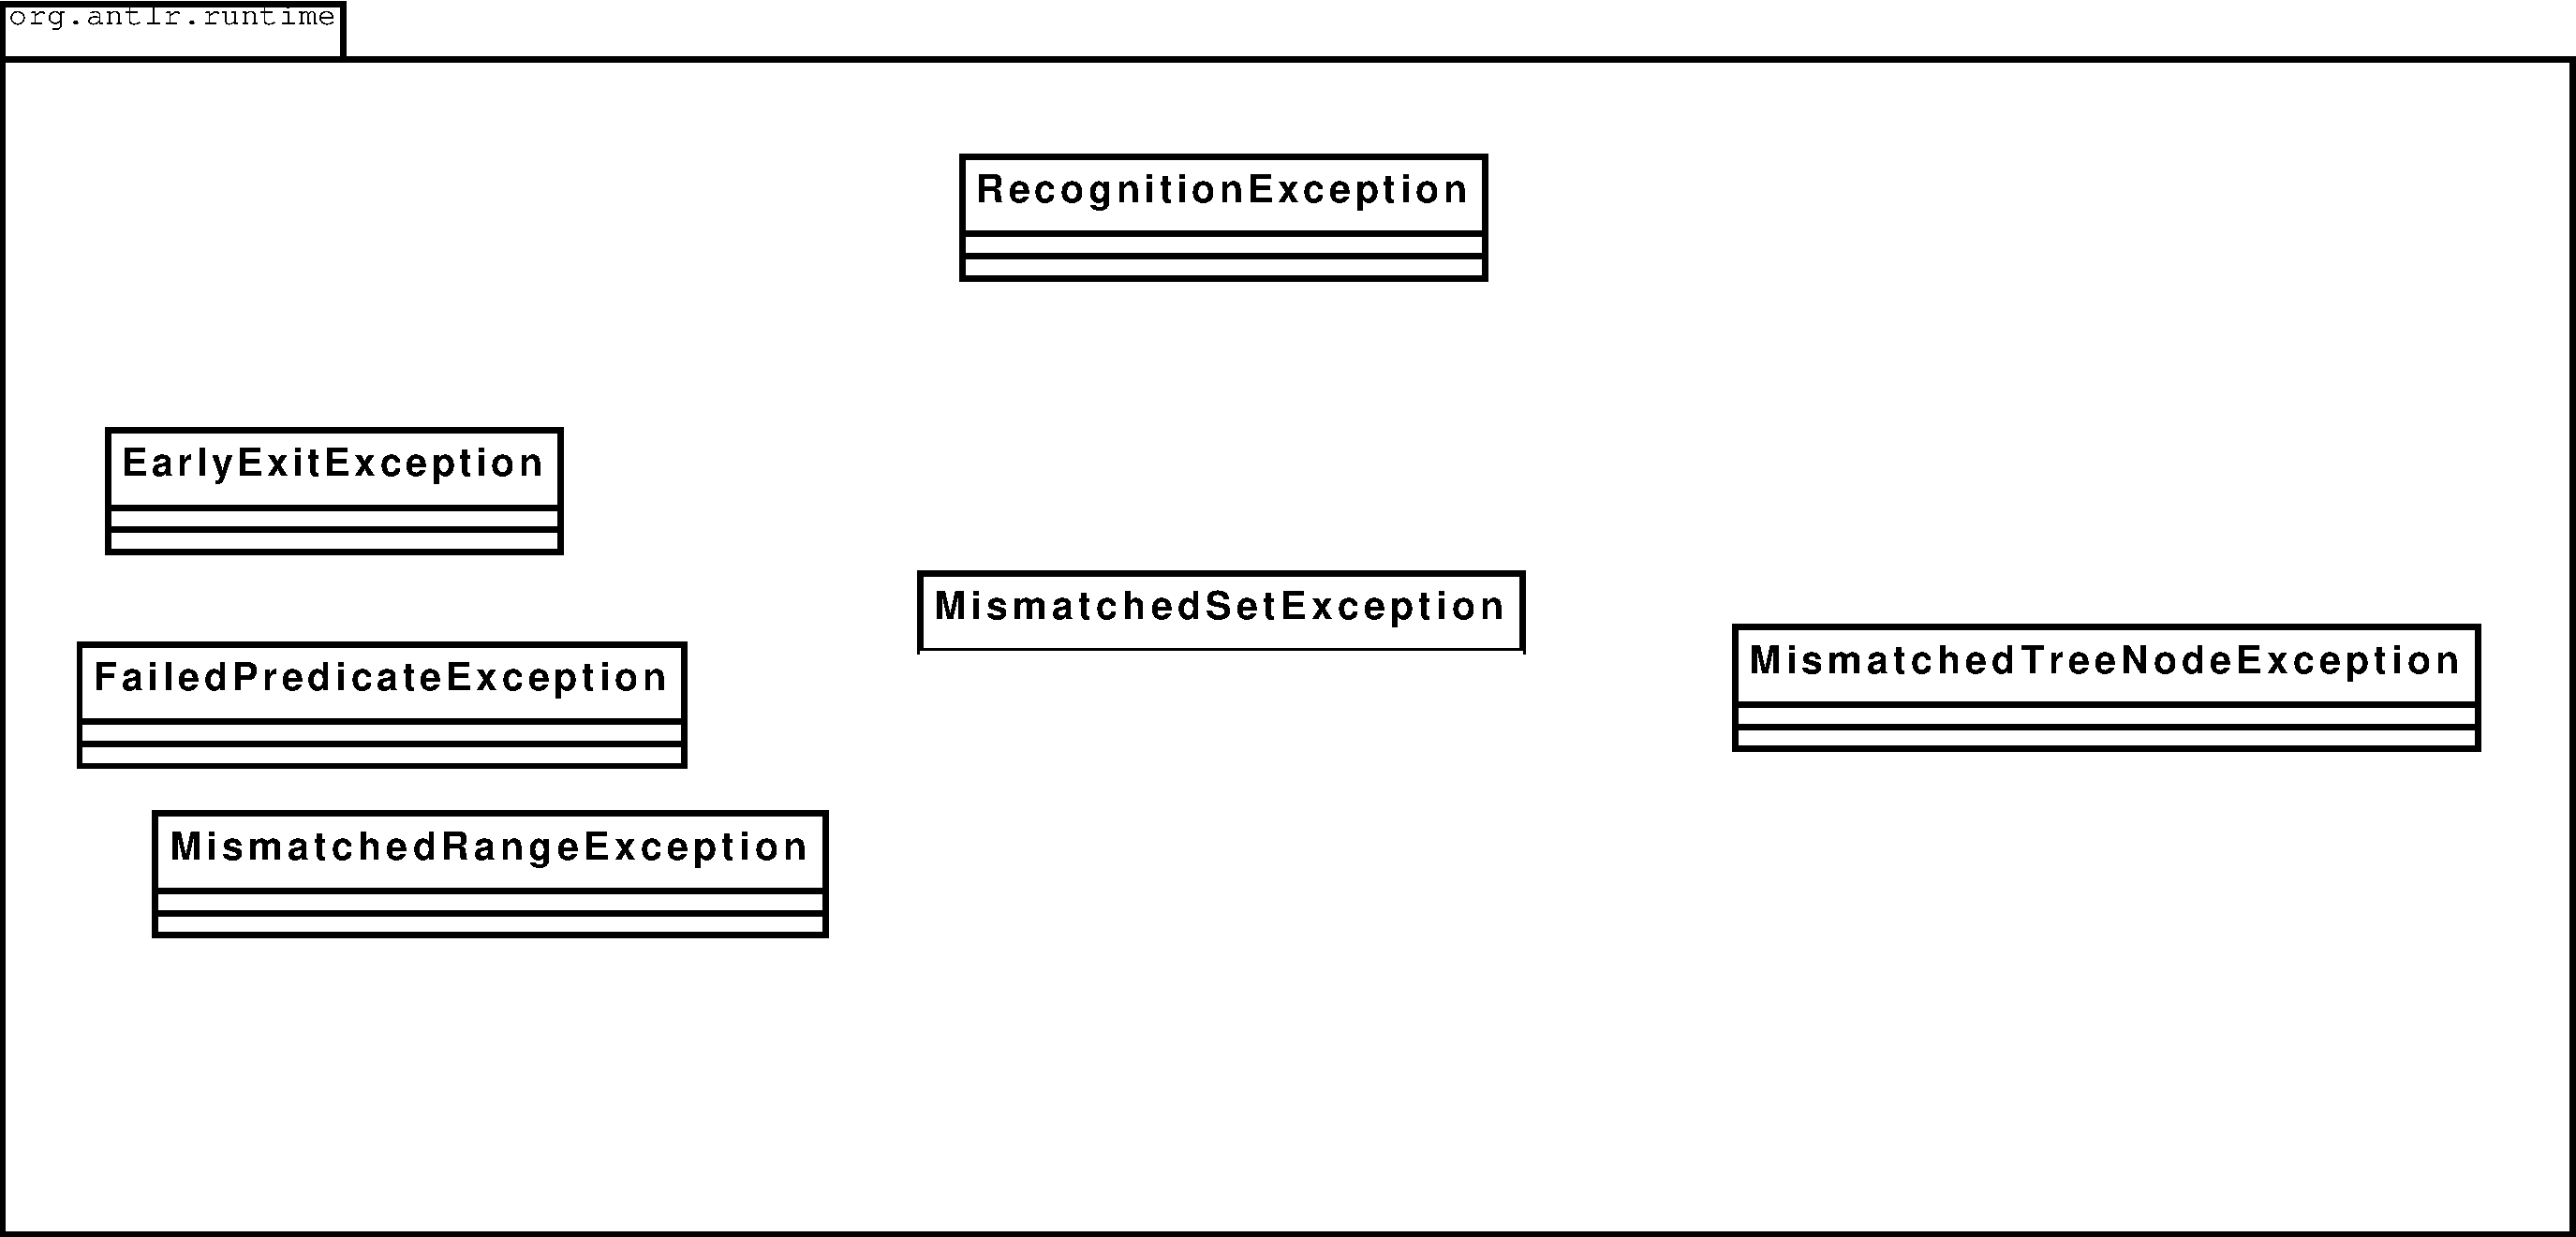
\includegraphics[width=1\textwidth]{diagrams/exception_uml}
  \caption{ANTLR exceptions class hierarchy}
\label{fig:antlrException}
\end{figure}
Error handling in ANTLR is initially done by catching exceptions and printing
an error message to stderr. The parser will then attempt to recover from the
error and continue parsing. This behaviour is not always desirable, so certain
methods were overridden to allow exceptions to be thrown upwards the stack to
the program that initiated the parser (the calling program, or top-level
program). An overview of the posible exceptions ANTLR can throw is shown in figure \ref{fig:antlrException}.

Specifically, this was done by overriding the methods \verb!mismatch()! as well as
\verb!recoverFromMismatchedSet()!, as such:

\begin{Verbatim}
    protected void mismatch(IntStream input, 
                            int ttype, 
                            BitSet follow)
        throws RecognitionException
    {
        throw new MismatchedTokenException(ttype, input);
    }

    public void recoverFromMismatchedSet(IntStream input, 
                                         RecognitionException e, 
                                         BitSet follow)
        throws RecognitionException
    {
        throw e;
    }
\end{Verbatim}

Additionally, a special \verb!@rulecatch! rule had to be added to force ANTLR from
handling errors and instead throwing the exceptions upwards:

\begin{Verbatim}
@rulecatch {
    catch (RecognitionException e) {
        throw e;
    }
}
\end{Verbatim}

However, some exceptions thrown by the lexer were impossible to handle - these
were handled in the \verb!nextToken()! method in the \verb!Lexer! superclass.
This issue has been documented in section 
\ref{sect:error_handling:syntax_errors}.


\section{Scope andz Typecheckz}

\underline{\textbf{\LARGE //TODO: Andreas}} Saksa det her fra future work... kan det bli mer diskusjon i stedet? Evt ogs\aa~dele det opp i to sections...

\subsubsection{Type Checking}
Currently the parser will not perform type checking on the parsed queries. This
is an essential feature and will be necessary to implement for the parser to be
applicable in any realistic setting. A type checking system with proper type
inference and synthesis could be a complex feature to implement in a language
such as XQuery, and might require considerable effort, especially in quality
assurance. 

\subsubsection{Scoping and Symbol Tables on AST}
Currently the scoping and symbol tables are being used directly in the grammar -
that is, during parse time. It would be benefitial to move this into being
performed in run time, and combine with type checking functionality.

\underline{\textbf{\LARGE //ODOT:}}

\section{Dead Ends}
\label{sect:discussion:deadEnds}
\underline{\textbf{\LARGE //TODO: Mads, om ikke du har noen p\aa~lager?}}



Hva har vi gjort som m\aa tte gj\o res om igjen?

\begin{itemize}
\item Skrive om dash: Validerende semantiske predikat, saa CharNotMinus etc
\item Feil splitting Lexer vs Parser, mye feilmeldingjakt
\item Keywords deklarert i @tokens -> vant alltid.
\item NCName med syntaktiske predikat
\end{itemize}

/* Hentet fra implementation: \\
In the grammar specified by the W3C, all the productions (terminals and
non-terminals) all start with uppercase letters. Initially this caused some
confusion, because this grammar naturally generated a very big lexer and a very
small and non-functional parser. \\
*/

\underline{\textbf{\LARGE //ODOT:}}